\documentclass[12pt]{article}
\usepackage{fancyhdr}     % Enhanced control over headers and footers 
\usepackage[T1]{fontenc}  % Font encoding
\usepackage{mathptmx}     % Choose Times font 
\usepackage{microtype}    % Improves line breaks      
\usepackage{setspace}     % Makes the document look like horse manure 
\usepackage{hyperref}
\hypersetup{
	colorlinks   = true, %Colours links instead of ugly boxes
	urlcolor     = blue, %Colour for external hyperlinks
	linkcolor    = black, %Colour of internal links
	citecolor   = black %Colour of citations
}
\usepackage{graphicx}
\usepackage{subcaption}
\usepackage{endnotes}
\usepackage{float}
\usepackage{algorithm}
\usepackage{algpseudocode}
\usepackage{multicol}
\usepackage{tikz}
\usetikzlibrary{snakes}
\usepackage{rotating}
\usetikzlibrary{positioning,shapes.multipart}

\usepackage[style=apa,backend=biber,citestyle=numeric]{biblatex}
\addbibresource{../refs.bib}

\title{Bayesian Neural Networks}
\author{
	Blair, Taylor
	\and
	Sorgmon, Ava
	\and
	Conor
}
\date{\today}
\let\footnote=\endnote

\usepackage{verbatim}

\pagestyle{fancy} % Default page style 
\lhead{Blair, Sorgman, Conor}
\chead{}
\rhead{\thepage}
\cfoot{}
\rfoot{}
\renewcommand{\headrulewidth}{1pt}
\renewcommand{\footrulewidth}{1pt}
\renewcommand{\theendnote}{\Roman{endnote}} 



\begin{document}
\doublespacing
\maketitle



\begin{abstract}
	Bayesian Neural Networks are...
\end{abstract}

\tableofcontents

\section{Introduction}




\subsection{History}

\begin{figure}[H]
	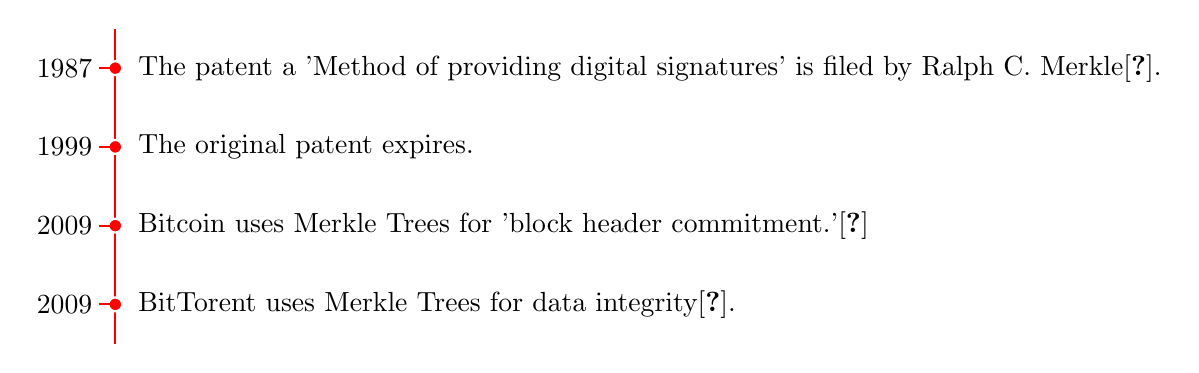
\begin{tikzpicture}[scale=0.5,every node/.style={outer sep=5pt}]
		%Notation: {year, the title of the event}
		%NOTE! Everyting is zero-based
		\def\ourInfo{{
				{"1987"," The patent a 'Method of providing digital signatures' is filed by Ralph C. Merkle\cite{merkle-patent}."},
				{"1999","The original patent expires."},
				{"2009","Bitcoin uses Merkle Trees for 'block header commitment.'\cite{friedenbach_alm_2017}"},			
				{"2009","BitTorent uses Merkle Trees for data integrity\cite{bep30}."},
		}}
		\pgfmathsetmacro{\length}{3}% Zero based.
		
		% Loop through the array containing all events.
		\foreach \i in {0, ..., \length}{
			\pgfmathsetmacro{\year}{\ourInfo[\i][0]}% Get the left cell (year)
			\pgfmathsetmacro{\eventName}{\ourInfo[\i][1]}% Get the right cell (event name)
			\draw[thick,red] (0,-2*\i-2)--(0,-2*\i);% Draw vertical line
			\ifnum \i=0 % Should be in red text
			\draw(0,-2*\i-1) node[black, right, align = left]{\eventName};% Display the event name
			\draw(0,-2*\i-1) node[black, left] {\year};
			\else % Should be in black text
			\draw(0,-2*\i-1) node[right, black]{\eventName};% Display the event name
			\draw(0,-2*\i-1) node[left] {\year};% Display the year
			\fi
		}
		% Draw the bullet with the dash
		\foreach \i in {0, ..., \length}{
			\filldraw[draw = white, fill = red,thick] (0,-2*\i-1) circle (5pt);
			\draw[thick,red] (-12pt,-2*\i-1)--(0,-2*\i-1);
		}
	\end{tikzpicture}
\end{figure}
	
	
\section{Neural Network}

\begin{figure}[H]
	\centering
	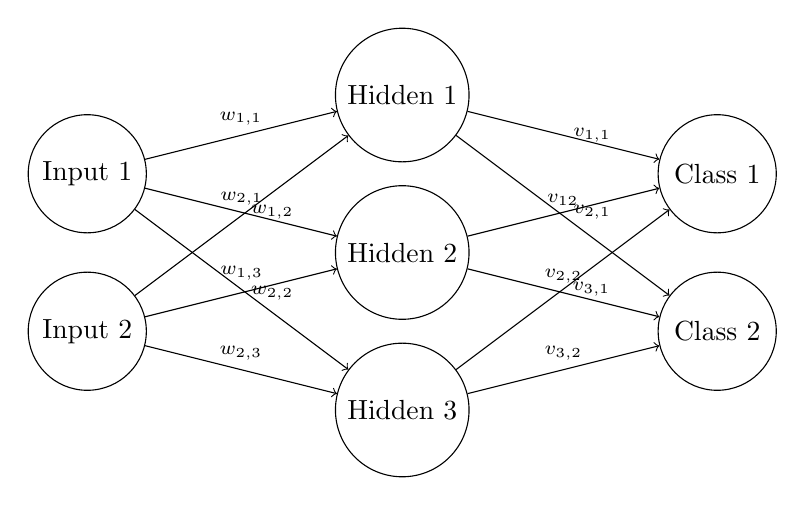
\begin{tikzpicture}
		% Define node styles
		\tikzstyle{neuron} = [circle, draw, minimum size=1.5cm];
		\tikzstyle{weight} = [font=\scriptsize];
		
		% Input layer (2 neurons)
		\node[neuron] (input1) at (-2,1) {Input 1};
		\node[neuron] (input2) at (-2,-1) {Input 2};
		
		% Hidden layer (3 neurons)
		\node[neuron] (hidden1) at (2,2) {Hidden 1};
		\node[neuron] (hidden2) at (2,0) {Hidden 2};
		\node[neuron] (hidden3) at (2,-2) {Hidden 3};
		
		% Output layer (2 neurons for classification)
		\node[neuron] (output1) at (6,1) {Class 1};
		\node[neuron] (output2) at (6,-1) {Class 2};
		
		% Connections with weights
		\draw[->] (input1) -- node[weight, above] {$w_{1,1}$} (hidden1);
		\draw[->] (input2) -- node[weight, above] {$w_{2,1}$} (hidden1);
		\draw[->] (input1) -- node[weight, right] {$w_{1,2}$} (hidden2);
		\draw[->] (input2) -- node[weight, right] {$w_{2,2}$} (hidden2);
		\draw[->] (input1) -- node[weight, above] {$w_{1,3}$} (hidden3);
		\draw[->] (input2) -- node[weight, above] {$w_{2,3}$} (hidden3);
		\draw[->] (hidden1) -- node[weight, right] {$v_{1,1}$} (output1);
		\draw[->] (hidden2) -- node[weight, right] {$v_{2,1}$} (output1);
		\draw[->] (hidden3) -- node[weight, right] {$v_{3,1}$} (output1);
		\draw[->] (hidden1) -- node[weight, above] {$v_{12}$} (output2);
		\draw[->] (hidden2) -- node[weight, above] {$v_{2,2}$} (output2);
		\draw[->] (hidden3) -- node[weight, above] {$v_{3,2}$} (output2);
	\end{tikzpicture}
	\caption{Example neural network}
\end{figure}

Neural networks....


Neural networks are made out of a series of neurons. 
\begin{figure}[H]
	\centering
	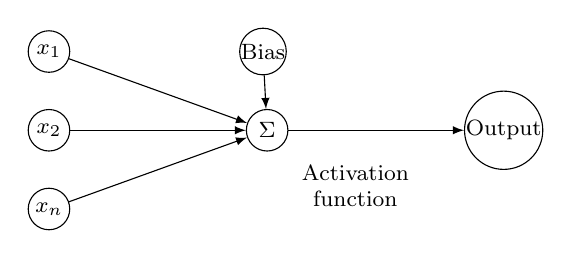
\begin{tikzpicture}[
		neuron/.style={
			circle,
			draw,
			minimum size=1.5em,
			inner sep=0pt,
		},
		font=\footnotesize,
		>=latex
		]
		% Draw the neuron
		\node [neuron] (neuron) at (0,0) {$\Sigma$};
		% Draw the input nodes and labels
		\foreach \i/\txt in {1/$x_1$,2/$x_2$,3/$x_n$} {
			\node [neuron,left=of neuron] (input\i) at (-1.5,-\i +2) {\txt};
			\draw[->] (input\i) -- node[above] {} (neuron);
		}
		% Draw the bias node and label
		\node [neuron,left=of neuron] (bias) at (1.25,1) {Bias};
		\draw[->] (bias) -- node[right] {} (neuron);
		% Draw the activation function label
		\node[align=center,below right =0.5em of neuron] {Activation \\ function};
		% Draw the output node and label
		\node [neuron,right=of neuron] (output) at (1.5,0) {Output};
		\draw[->] (neuron) -- node[above] {} (output);
		% Draw the relevant functions
		%\draw[->] (0,-1.5) -- (0,-2.5) node[midway,right] {Weighted sum};
		%\draw[->] (-1.5,-3.5) -- (-1.5,-4.5) node[midway,left] {Bias};
		%\draw[->] (1.5,-0.5) -- (1.5,-1.5) node[midway,right] {Activation};
		
		% Draw the activation function shape
		%\node[draw,rectangle,minimum width=2em,minimum height=2em] (actfunc) at (0,1) {};
		%\node[above=0.1em of actfunc] {ReLU};
		
	\end{tikzpicture}
	\caption{Neural network neuron}
\end{figure}

\subsection{Convolutional Neural Networks }

\begin{figure}[H]
	\centering
	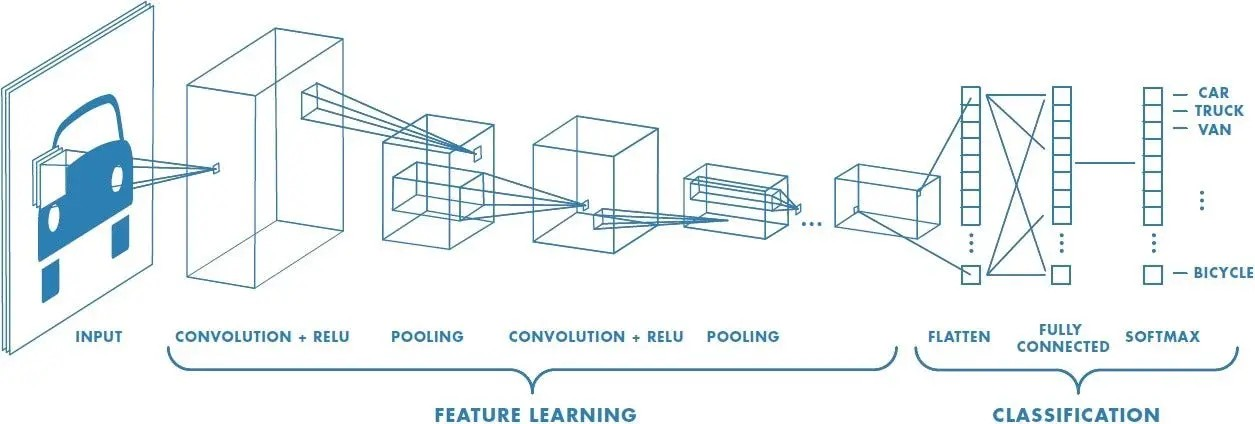
\includegraphics[width=.8\textwidth]{../Images/big-pic-cnn.jpg}
	\caption{CNN pipeline \cite{eli5CNN}}
\end{figure}

Convolutional neural networks (CNN) are a type of neural network that is better suited for image recognition. Instead of reading the entire image a CNN slides over the image... 

The result is that the neural network trains faster..

\section{Bayesian Neural Networks}

\begin{figure}[H]
	\centering
	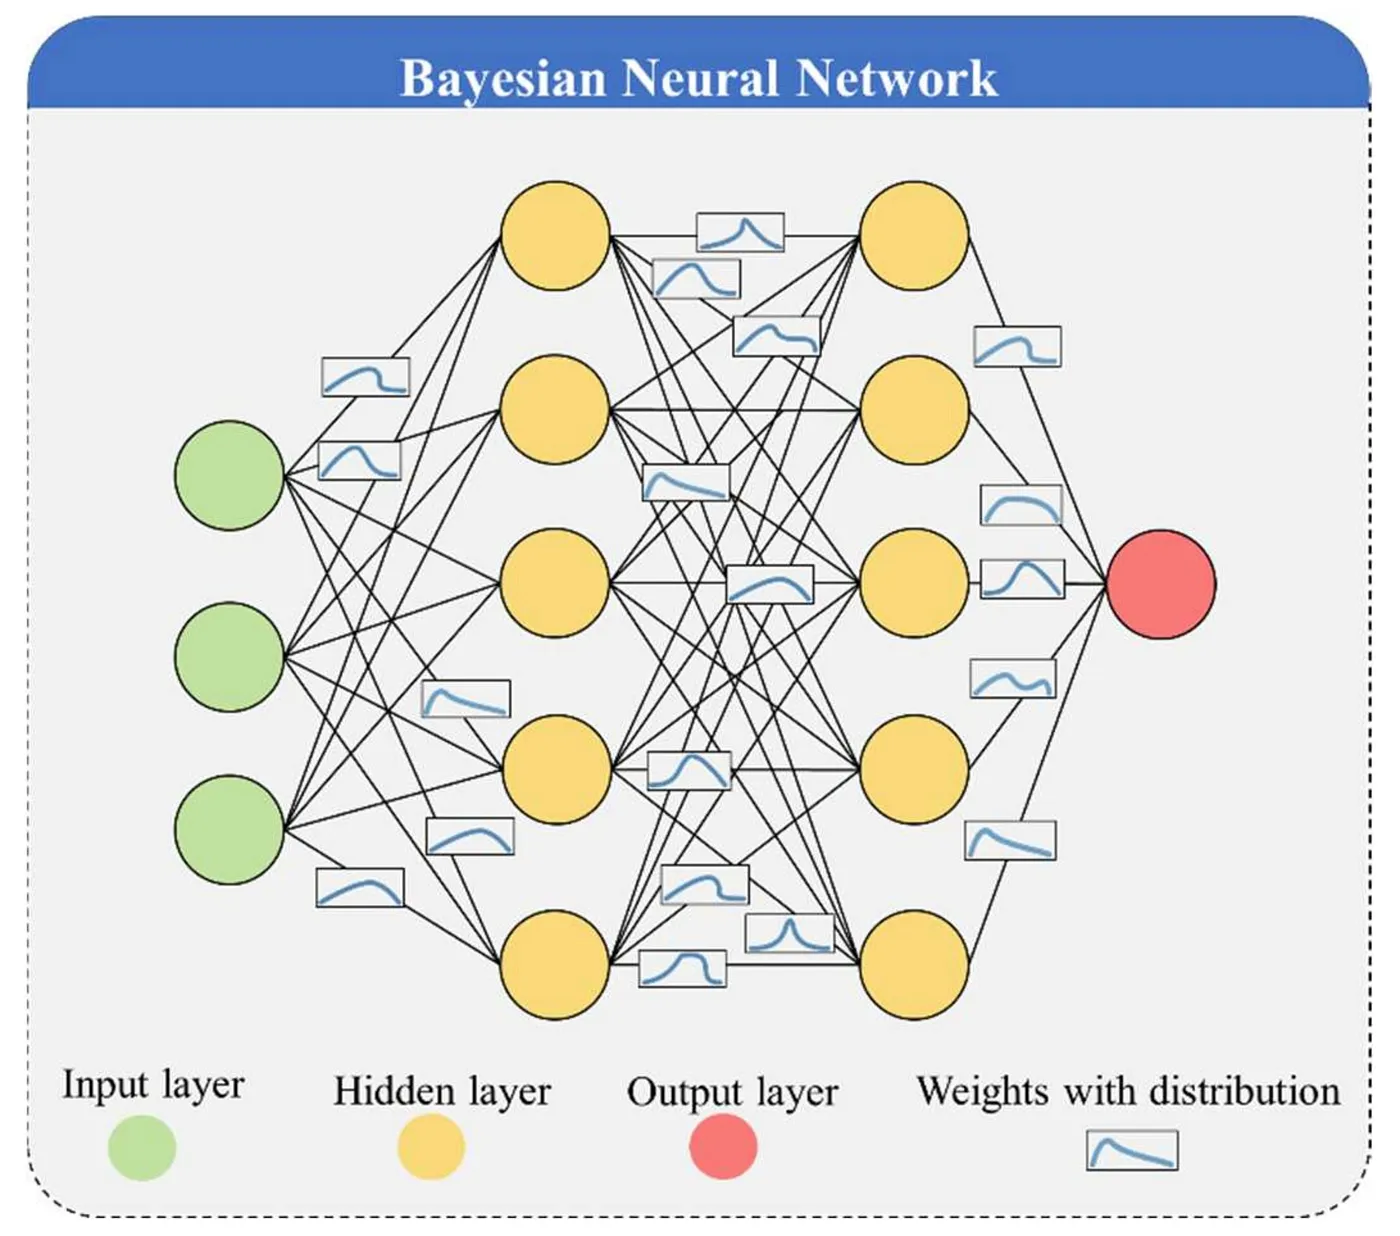
\includegraphics[width=.55\textwidth]{../Images/example_bnn.png}
	\caption{Example BNN  \cite{FleszarBNN}}
\end{figure}

Bayesian neural networks take the same principle as 

Similar to a Neural network such as... 

\begin{figure}[H]
	\centering
	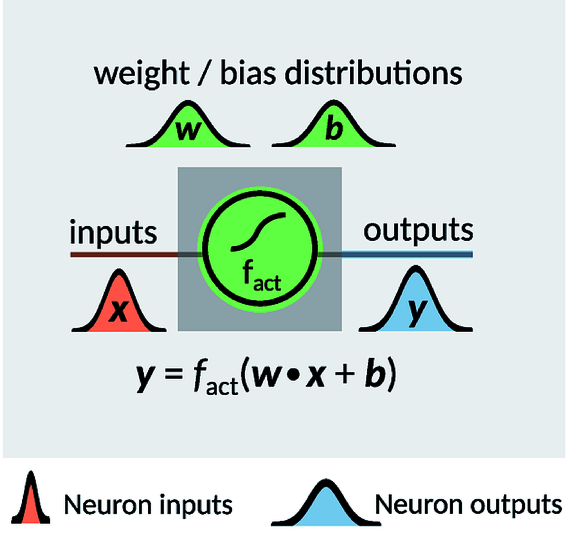
\includegraphics[width=.55\textwidth]{../Images/BNN-neuron.png}
	\caption{Example BNN Neuron \cite{hase2019machine}}
\end{figure}

\subsection{Bayesian Conolutional Neural Networks}

Same principle...

\section{Simulation}

We use a BCNN implementation from \href{https://github.com/kumar-shridhar/PyTorch-BayesianCNN}{Github} based on work from ... \cite{shridhar2019comprehensive} \cite{shridhar2018uncertainty}

\subsection{CIFAR-10}

	\begin{figure}[H]
		\centering
	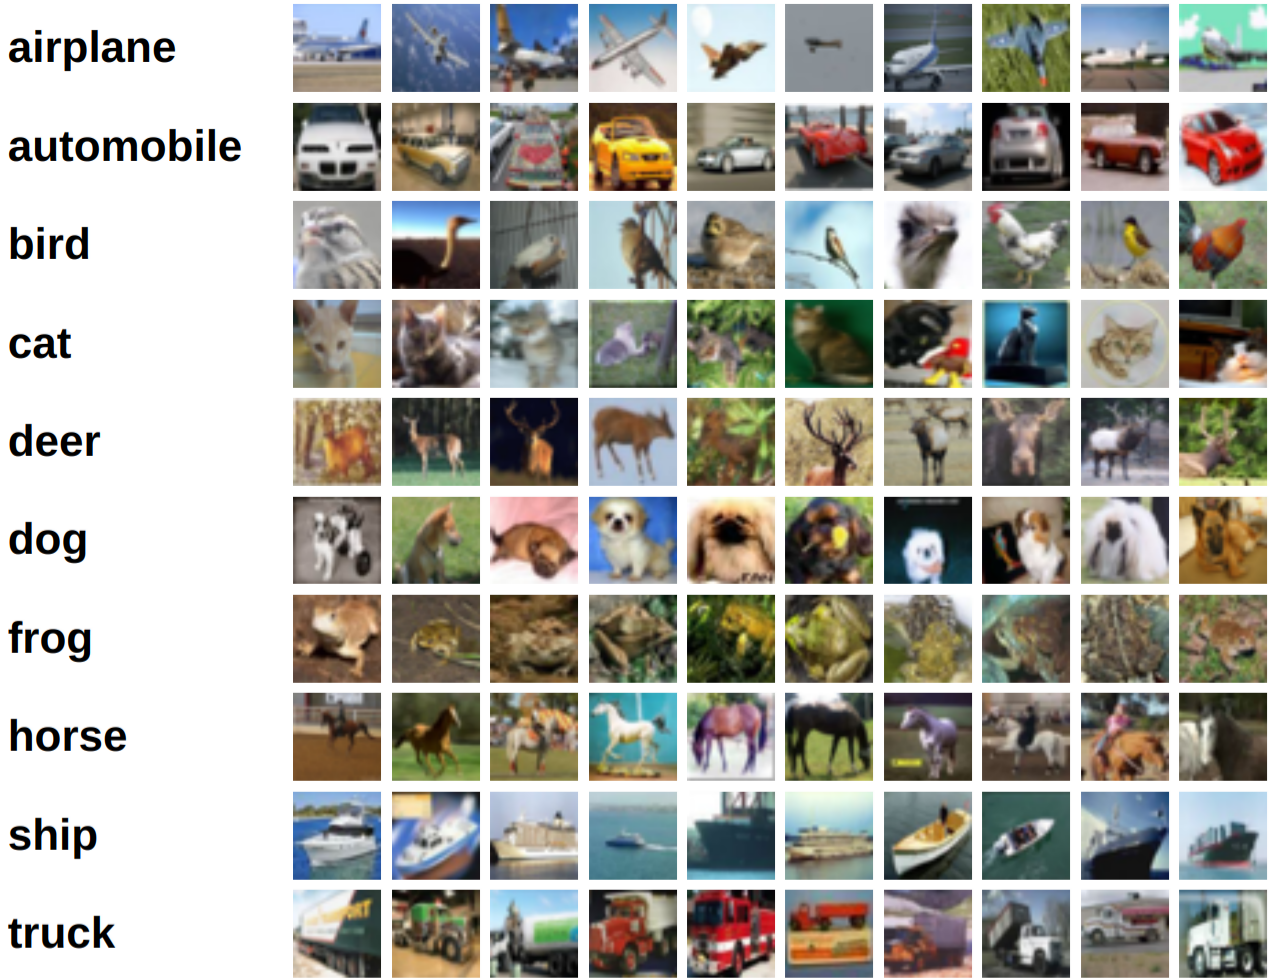
\includegraphics[width=.75\textwidth]{../Images/cifar-10.png}
	\caption{Example CIFAR-10 images \cite{cifar10}}
\end{figure}

The CIFAR-10 dataset...


\subsection{Hyperparamaters}

We used the following hyperparamaters for training
	\begin{center}
		\begin{tabular}{|c||p{3cm}|p{3cm}|} % Adjust p{width} as needed
			\hline
			\textbf{Hyperparameter} & \textbf{CNN} & \textbf{BCNN} \\ [0.5ex] 
			\hline\hline
			Epochs & 500 & 500\\
			\hline
			Learning Rate & ....  & May be higher (0.01 - 0.1) due to simpler structure  \\
			\hline
			Regularization & L1/L2 weight decay or Dropout common to prevent overfitting & Can benefit from Dropout, but weight decay might be less crucial \\
			\hline
			Optimizer & Adamw  & Adamw  \\
			\hline
		\end{tabular}
	\end{center}
	

\subsection{Results}

\begin{figure}[H]
	\centering
	\begin{subfigure}{.5\textwidth}
		\centering
		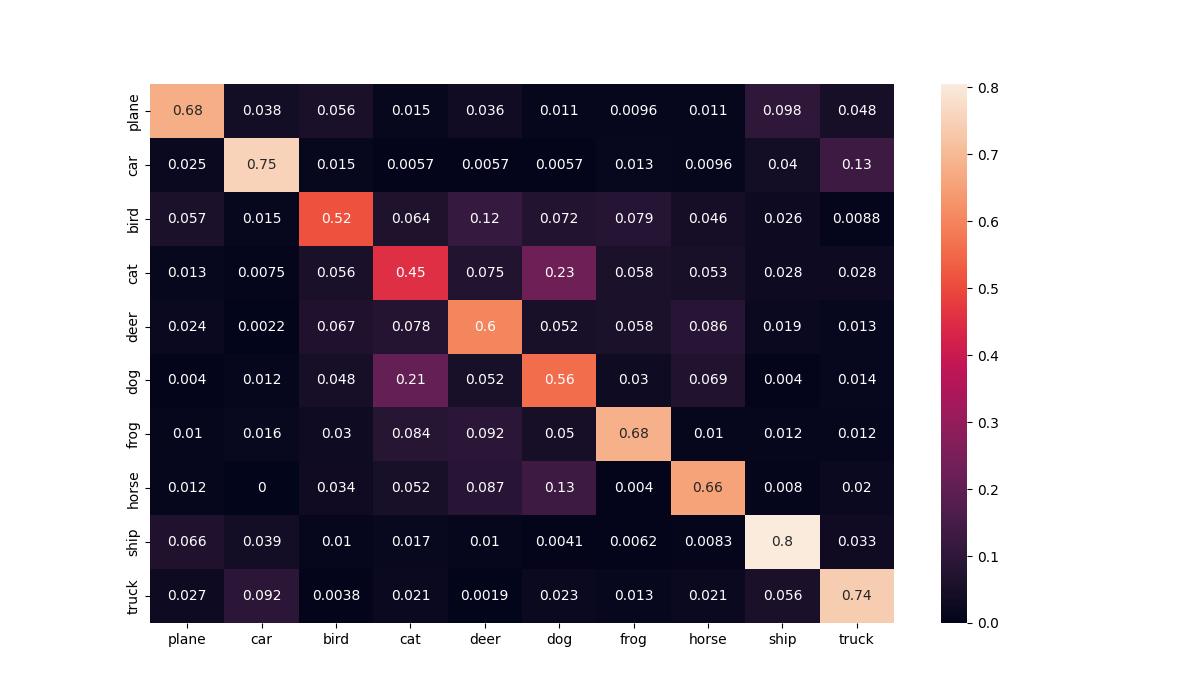
\includegraphics[width=.9\linewidth]{../Images/CNN_confusion_matrix}
		\caption{CNN}
	\end{subfigure}%
	\begin{subfigure}{.5\textwidth}
		\centering
		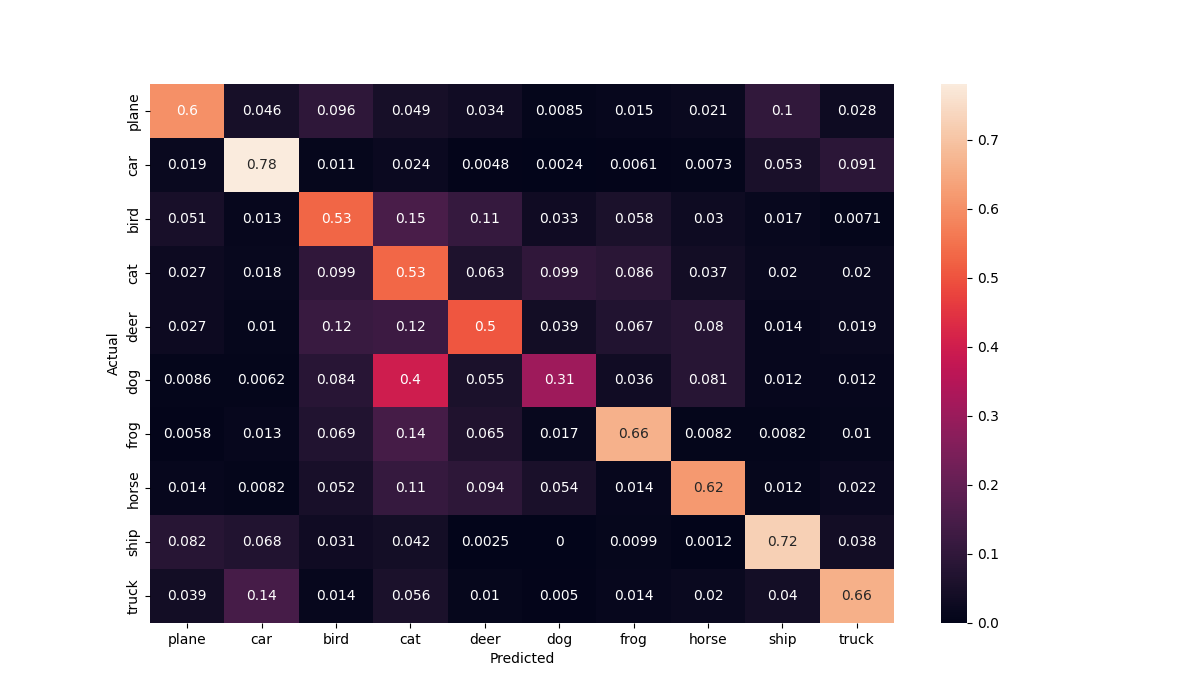
\includegraphics[width=.9\linewidth]{../Images/BNN_confusion_matrix}
		\caption{BCNN}
	\end{subfigure}
	\caption{Confusion matrices}
\end{figure}

\section{Closing}



\newpage

\printbibliography


\end{document}
